%%MAIN: thesis.tex

%%%%% The Solution %%%%%
\chapter{Proposed Solution: A New Teaching Environment for Programming} \label{ch_pa}

In order to let students have a \emph{Sichtenwechsel} with relation to programming, i.\,e. have them experience several different abstraction layers involved between a program's source code and its execution, a new teaching environment dubbed ``Processing Abstractions'' is proposed:

Within Glamorous Toolkit, we've implemented support for the Processing programming language and molded views for every implementation step along the way. This allows for creating interactive notebook pages containing source code and a variety of these views, showing e.\,g. the abstract syntax tree (AST) and resulting bytecode for the GT virtual machine side-by-side (see figure \ref{fig_gt_screenshot}).

In this chapter, we document the development of this environment and the reasons for the approaches chosen. If you want to try things out directly, see appendix \ref{app_setup} for how to install all referenced code\footnote{Remove the line \ct{GtExplorationHomeSection studentMode: true.} in order to also see our implementation notes.} A stable snapshot of the code discussed here is available on Github \cite[Bue25, Bue25a].



\section{Reasons for Using Processing and Glamorous Toolkit}

For the past decade, we've taught the introduction to programming using Processing to ninth graders. This consisted of an introduction into the language along relatively simple examples inspired by minimalist art and games (similar to the approach by Reas and Fry \cite{Rea14} described in \ref{ssc_top_down}). In a separate sequence, we've taught computer architecture in a bottom up approach (inspired by Nisan and Schocken \cite{Nis21} as described in \ref{ssc_bottom_up} but much abbreviated).

While the introduction to programming was usually quite well received by students and also led to satisfying results, the sequence on computer architecture did less so. The two sequences also didn't fit together as nicely as we'd have liked and processor and memory remained a mystery for too many students. Hence the decision to look into combining the two sequences.

At this point, we've briefly evaluated whether staying with Processing was reasonable. Reasons to do so were manyfold: As seen in \ref{sc_processing}, Processing allows a top down approach starting at visual arts, which allows to motivate students with less interest in mathematics and natural sciences; Processing also quickly yields pleasant looking results, which also adds to initial motivation \cite{Chi23}; then it can be based on still popular and widely used Python, which allows using it as a stepping stone and makes it a `real' programming language in the eyes of novices; on the other hand, Processing itself is sufficiently unknown that even students already experienced with programming will have something new to discover; additionally, Processing has a large community sharing sketches and ideas which can be used as inspiration for both students and teachers; finally, its proven itself in our own experience over the years.

While Modrow and Strecker prefer a block based language, we feel that at least parts of their issue with a text based programming language can be remedied by having a live environment with custom error messages. For remedying their remaining issue about allowing individual bits of code to be called independently, that could be achieved in one of the ways Glamorous Toolkit does this: either by offering separate playgrounds which do work similarly to a REPL; by allowing multiple code snippets to access the same environment (as it also works in Jupyter notebooks); or by allowing only selected code to be executed. The last option would be easiest to implement.\footnote{It hasn't been implemented for three reasons: At least in the beginning, it might confuse students more than it helps, which goes against manageability (see \ref{ssc_manageability}); most visual commands can't be executed entirely independently in Processing, as output always depends on \ct{size} and maybe other stateful commands; and interaction with the animation loop would have to be figured out: whether it's has to be paused during the entire interaction, just between two user commands or even not at all.}

Chiodini \emph{et al.} \cite{Chi23} also propose starting with visual programming but have different requirements: In order to keep an introductionary language manageable, they ask among others for a limited API which should be expandable by students (see also \ref{ssc_manageability}). And the full Processing API can indeed be quite overwhelming, so only a subset must be introduced at the start. Indeed also for this reason only a subset has been implemented in GT (see \ref{app_api}), although already including some seemingly unnecessary functions: E.\,g. the \ct{circle} function is easily implemented in terms of the more generic \ct{ellipse} function (see figure \ref{fig_circle}) -- either in the implementation of the Processing API or by students.

\begin{cfigure}[fig_circle]{Implementation of \ct{circle} as built-in API and in user code}
\begin{minipage}{.5\textwidth}
\begin{code}
ProcessingCanvas >> circle: x y: y d: d
	self
		ellipse: d
		by: d
		at: x @ y
\end{code}
\end{minipage}
\begin{minipage}{.45\textwidth}
\begin{code}
def circle(x, y, d):
	ellipse(x, y, d, d)
\end{code}
\end{minipage}
\end{cfigure}

Another requirement by Chiodini \emph{et al.} is for problems to be transparently decomposed and solutions recomposed. This is indeed an issue with Processing: Moving a composed shape to a different location requires adjusting the coordinates of all basic shapes involved, therefore variables and even functions have to be introduced sooner rather than latter to allow the examples shown \cite{Chi23} to work. Similar to how they introduce a library to achieve their desired API, the same functionality could be implemented on top of Processing at a later stage if desired.\footnote{In the provided teaching materials, an example of how to implement a simpler Turtle based API is provided (see ``Schildkr�ten und Rekursion'').}

The main reason for not introducing a new API as proposed by Chiodini \emph{et al.} is the same as the reason for not introducing an entirely new programming language optimized for teaching (as done e.\,g. by Black and Bruce \cite{Bla18}): This prevents benefiting from the large community and preexisting documentation and example code.

As development framework, Glamorous Toolkit was chosen for its moldable environment: As shown in \ref{sc_gt}, different views are quick to implement and can be combined freely with interactions and updates between them.

Of course, since GT is based on Smalltalk, an initial effort is required to learn language and environment before these benefits can be used. This is helped by Smalltalk's regular syntax and GT's reflection capabilities, which allows finding API, documentation and examples easily.\footnote{For Smalltalk and GT's ancestor Pharo, there are sufficient resources available online, for GT itself, there's the ``Glamorous Toolkit Book'' \cite{Gir23} and a Discord server.}

Implementing a new language in GT can happen along the moldable patterns documented in \ref{sc_moldable}: Starting with concrete samples, classes and views for handling them are molded in steps until the desired behavior is reached; then code is refactored into permanent methods on the one hand and a concrete example serving as test case on the other. Whenever the need for a different view into the program or one of its intermediary forms (such as AST, bytecode or output) arises, the view is constructed in the same way by first iteratively shaping the data into the desired form and then either passing this to one of GT's standard views (text, list, tree, table, forward) or composing the view's layout in the same way iteratively.



\section{Development of ``Processing Abstractions''}

Within Glamorous Toolkit, Processing is implemented through transpilation to Smalltalk. This allows reusing several of GT's libraries: \ct{PythonParser} for parsing Processing with Python syntax and \ct{OpalCompiler} for compiling Smalltalk with bytecode extractable through \ct{CompiledCode>>>symbolicBytecodes}.

Since Processing implemented on top of Python is a strongly but dynamically typed language, it maps well onto Smalltalk which is the same. Still, initially three other approaches were considered:

Processing could be run either in the original JRE and then accessed through Python or directly run using one of several Python libraries \cite{Tab22}. In all cases, its objects would be accessed through \ct{PythonBridge}. Since at the time of writing, support for PythonBridge under Windows was difficult to achieve in a portable manner (i.\,e. without requiring students to install multiple different packages which increases the risk of accidental breaking and thus potential support issues), this approach was rejected.

Alternatively, Processing could have been implemented through an interpreter in GT\footnote{Remnants of which are available as \ct{ProcessingInterpreter}}. This would have required to write a separate compiler for creating bytecode just for demonstration purposes. Instead, a compiler from Processing to Smalltalk bytecode could have been written.\footnote{A compiler for a tiny subset of Processing is included as \ct{ProcessingCompiler}.} While this would have allowed for closer control over optimizations, it would effectively have become a reimplementation of most of \ct{OpalCompiler}.


\subsection{Implemented Classes}

%%%%% The Solution (UML Diagram) %%%%%

\newgeometry{bottom=1cm}

\begin{landscape}

\begin{cfigure}[fig_uml_processing]{Diagram of most classes involved in running Processing code within \ac{GT}}

\begin{tikzpicture}

\begin{package}{Processing}

\begin{class}[text width=6cm]{ProcessingSource}{0, 0}
\operation{fromFile:}
\operation{fromPage:at:}
\operation{fromSnippet:}
\end{class}

\begin{class}[text width=6cm]{ProcessingProgram}{0, 2.5}
\operation{source:}
\end{class}

\begin{class}[text width=6cm]{ProcessingParser}{8, 0}
\operation{parse:}
\end{class}

\begin{class}[text width=6cm]{ProcessingTranspiler}{8, 2.5}
\operation{transpile:}
\end{class}

\begin{class}[text width=6cm]{ProcessingTranspilationSlice}{16, 0}
\operation{link:method:from:to:}
\end{class}

\begin{interface}[text width=6cm]{ProcessingCodeBase}{0, 5}
\operation{gtRun}
\end{interface}

\begin{class}[text width=6cm]{ProcessingRunner}{8, 5}
\operation{run:}
\operation{runSteps:}
\end{class}

\begin{class}[text width=6cm]{ProcessingCanvas}{0, 7.5}
\end{class}

\begin{class}[text width=6cm]{ProcessingCanvasPresenter}{8, 7.5}
\implement{ProcessingCanvas}
\end{class}

\begin{class}[text width=6cm]{ProcessingCanvasElement}{16, 7.5}
\end{class}

\begin{class}[text width=6cm]{ProcessingAstCleaner}{16, 2.5}
\operation{clean:}
\end{class}

\begin{interface}[text width=6cm]{ProcessingCanvasShape}{8, 9}
\end{interface}

\begin{class}[text width=6cm]{ProcessingRunStep}{16, 5}
\operation{clean:}
\end{class}

\draw[umlcd style dashed line, ->] (ProcessingSource) -- node[black]{program} (ProcessingProgram);
\draw[umlcd style dashed line, <->] (ProcessingProgram) -- node[black, sloped]{ast} (ProcessingParser);
\draw[umlcd style dashed line, ->] (ProcessingProgram) -- node[black]{(source:)} (ProcessingTranspiler);
\draw[umlcd style dashed line, ->] (ProcessingTranspiler) -- node[black, sloped]{compile:} (ProcessingCodeBase);
\draw[umlcd style dashed line, <->] (ProcessingTranspiler) -- node[black]{(transpile:)} (ProcessingAstCleaner);
\draw[umlcd style dashed line, ->] (ProcessingTranspiler) -- node[black, sloped]{(compile:)} (ProcessingTranspilationSlice);
\draw[umlcd style dashed line, ->] (ProcessingProgram) -- node[black]{compilation} (ProcessingCodeBase);
\draw[umlcd style dashed line, ->] (ProcessingProgram) -- node[black]{run} (ProcessingRunner);
\draw[umlcd style dashed line, ->] (ProcessingRunner) -- node[black]{runStepwise:} (ProcessingRunStep);
\draw[umlcd style dashed line, ->] (ProcessingCodeBase) -- node[black]{gtCanvas} (ProcessingCanvas);
\draw[umlcd style dashed line, ->] (ProcessingCanvas) -- node[black]{presenter} (ProcessingCanvasPresenter);
\draw[umlcd style dashed line, ->] (ProcessingCanvasPresenter) -- node[black]{canvasElement} (ProcessingCanvasElement);
\draw[umlcd style dashed line, ->] (ProcessingCanvas) -- node[black, sloped]{(draw)} (ProcessingCanvasShape);
\draw[umlcd style dashed line, <-] (ProcessingCanvasShape) -- node[black, sloped]{asElement} (ProcessingCanvasElement);

\end{package}

\end{tikzpicture}

\end{cfigure}

\end{landscape}

\restoregeometry


\begin{todo}
\item Shorten this chapter, move the details into an appendix
\end{todo}


The product consists of the following main classes which can be found in GT through the spotter (\faSearch):

\ct{ProcessingCanvas} provides the implementation of most of the Processing API for rendering the various shapes in the form of \ct{BlElement}s (wrapped through \ct{ProcessingCanvasShape}). It does this through \ct{ProcessingCanvasPresenter} into a \ct{ProcessingCanvasElement} of which there can be multiple, allowing to use a canvas for multiple views. The canvas also provides access to the individual shapes and all of its state. Rendering onto the canvas happens through the transpiled and compiled Processing program for which a new canvas is created for every separate run.

Processing programs can be written either inside GT's notebook in form of a ``Processing/Python'' snippet, in form of a Smalltalk string or in separate files. All forms are loaded through the \ct{ProcessingSource} class. Since we mostly want Processing source and its various views to be seen in a notebook page, the most common way to process a Processing program will be inside the page through\footnote{The \ct{at: 1} part of the message may also be omitted, if there's only one snippet on a notebook page. Omit the \ct{renderLive} message, if you want access to any of the intermediary states or different views.}
\begin{code}
(ProcessingSource fromPage: thisSnippet page at: 1) renderLive
\end{code}

For a pure introduction to programming, it's even enough to rely on the Processing snippet to produce output, as that allows for the most common forms of output:

\begin{itemize}
\item {\small\faPlay} (or its shortcut \ct{Ctrl+R} for ``Run'') runs the program and either display its visual output or an inline error message.
\item {\small\faPlay}\texttt{i} (or its shortcut \ct{Ctrl+G} for ``debuG'') runs the program, recording all individual steps at the level of (nested) Python expressions -- allowing to step through the program and inspecting among others the values of variables and the current state of the output.
\item {\small\faPlay}\texttt{a} (or its shortcut \ct{Ctrl+D} for ``Details'') shows the program in its main decomposed states: source, abstract syntax tree, bytecode and output.
\item \lightning\ (or its shortcut \ct{Ctrl+Shift+D}) opens GT's Smalltalk debugger at the \ct{gtRun} entry point of the transpiled code for live debugging for either advanced students or for looking under the hood of the API calls.
\end{itemize}

The snippet is implemented in \ct{LeProcessingSnippet} which builds upon GT's \ct{LePythonSnippet} for syntax highlighting but accesses Processing through \ct{ProcessingSource} instead of Python through \ct{PythonBridge}.

For embedding output or any other view inside a notebook page, an ``Element'' is added with either the code from above or with \ct{renderLive} replaced with \ct{renderLiveView:} with the symbol of the desired view appended (\ct{#gtTreeFor:}, \ct{#gtTranspilationFor:}, \ct{#gtBytecodeFor:}, \emph{etc.}; see the ``views'' category of \ct{ProcessingSource} and \ct{ProcessingProgram} for all available views).

For all the views, a \ct{ProcessingProgram} is created through \ct{ProcessingSource>>>program} which transforms it into its various forms:

\begin{itemize}
\item \ct{ProcessingParser} is used for parsing the source into an AST. Since Processing shares Python's syntax, the parser is a very thin wrapper around GT's \ct{PythonParser}. The AST is then slightly modified through \ct{ProcessingAstCleaner} to better map Python to Smalltalk: Since statements after a \ct{return} are allowed in Python but not supported in Smalltalk, they're silently dropped (a warning about unreachable code could be added); and parenthesized expressions are parsed into \ct{PyTupleExpressionNode} which complicate later optimizations with relation to operator chains, in particular logical operators \ct{and} and \ct{or}.
\item \ct{ProcessingTranspiler} then walks through the cleaned AST and transpiles Python expressions to the corresponding Smalltalk, recording a \ct{ProcessingTranspilationSlice} for every (sub)expression, thus later allowing to map bytecode its mapping into Smalltalk code back to the corresponding Processing source. If \ct{setup} and/or \ct{draw} functions are defined in Processing code, the implicit animation loop is added to the end of top-level code. Processing API calls -- if not overwritten by user code -- are translated through messages of the form \ct{ProcessingTranspiler>>>emit_...:} which the transpiler detects through reflection.
\item The transpiled code is compiled to methods of an anonymous subclass of \ct{ProcessingCodeBase}. This base class provides views at the lower abstraction levels from transpiled code to bytecode and also the entry point to the user supplied program \ct{gtRun} which contains top-level code. Global variables are turned into instance variables, thus being available to all Processing functions in the form of Smalltalk methods.\footnote{In order to prevent overriding of \ct{gtRun} and the different view messages, Processing names starting with \ct{gt} are renamed to starting with \ct{gt_} during transpilation.}
\end{itemize}

While compiled Processing programs can be run directly, \ct{ProcessingRunner} is used for ensuring the presence of an output canvas, for allowing program execution to be interrupted and for extracting \ct{ProcessingRunStep} instances for every Processing (sub)expression.

From these, \ct{ProcessingProgram} provides all views corresponding to Processing code and combined views. In order not to overwhelm students with too many views, \ct{gtDefaultInspectorTool} has been implemented for hiding all but the main four views behind the same symbols as used by the snippet.

During compilation, most common exceptions are \ct{SmaCCParserError} during parsing, \ct{ProcessingCompileTimeException} during transpilation and \ct{ProcessingRunTimeException} during execution. At this point, exceptions occurring in the transpiled code are not translated yet. Since most programs are meant to be re-run live, a heuristic has been implemented for catching endless loops which may naturally occur while a program's source is modified where e.\,g. a variable's value is modified but at the end of a \ct{while} loop. Instead of detecting the endless loop from code, runtime has been restricted to a maximum of two seconds for non-animated programs and thirty seconds for animated programs.


\subsection{Implemented Views}

Since the goal of this product was showing various states of a program in a way that can be explored live, may different views into the classes listed above have been implemented. These views are all available either from \ct{ProcessingProgram} or through \ct{ProcessingSource>>>renderLiveView:}. Note that the convention is that any view has a name of the form \ct{gt...For:}, is categorized as ``views'' (and of course has a \ct{<gtView>} annotation).

At the level of source code, there's three different views showing the source with syntax highlighting (\ct{gtContentsFor:}), showing the individual source characters with their unicode value (\ct{gtSourceCharsFor:}), and showing the bytes as they would be written to disk, assuming the default UTF-8 encoding also used by the original Processing IDE, with bytes also displayed in hexadecimal and binary notations (\ct{gtSourceBytesFor:}). With these views and suitable sample code, students might be able to deduce some regularities with relation to ASCII character ranges and UTF-8 encoding.

As most of the available views, these views can be combined, so that students can navigate one view and compare the selected character or byte with its position in the source code. Sensible combinations such as \ct{gtSourceBytesPlusSourceFor:} are provided, others can be created as desired on the basis of the provided ones. Using the helper class \ct{ViewComparison}, the same view for multiple programs can also be linked for side-by-side comparison.

For the parsing phase, there's another three views showing either just the tokens after the lexing phase, including line number and indentation (\ct{gtTokensFor:}), showing the abstract syntax tree as a tree list with purely structural tokens visually distinguished (\ct{gtTreeFor:}), and showing the abstract syntax tree layed out horizontally using GT's Mondrian library (\ct{gtTreeMondrianFor:}). All of these views can again adjust live to code changes, allowing students to explore how tokenization and parsing might work by modifying source code and hypothesizing (see figure \ref{fig_views_parser}).

\begin{cfigure}[fig_views_parser]{Screenshot of a page of student content showing modifyable Processing source with live views for tokenization (left) and abstract syntax tree (right).}
\centering
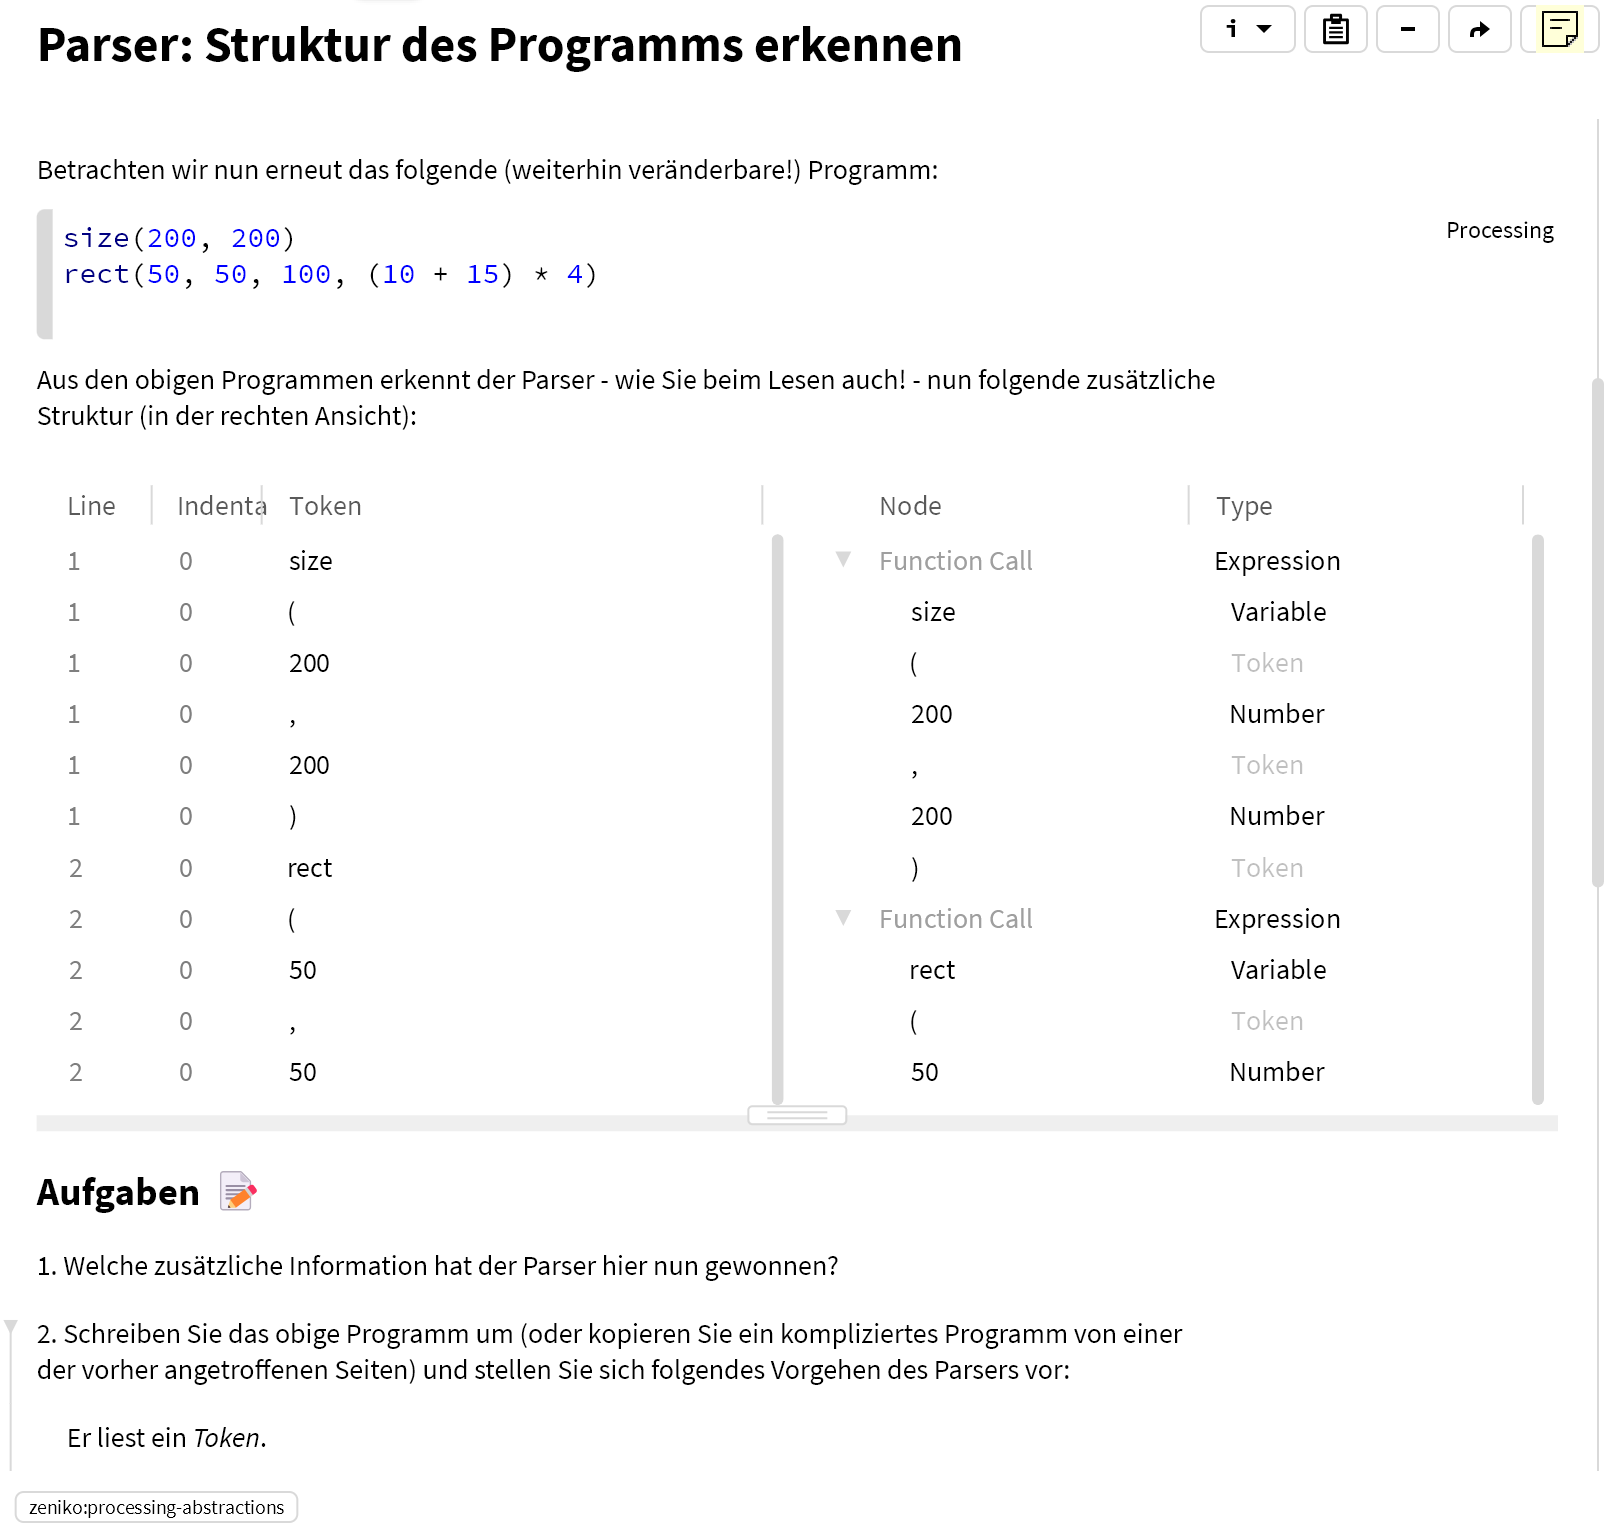
\includegraphics[width=.8\textwidth]{screenshot_parser}
\end{cfigure}

The view \ct{gtTranspilationFor:} allows on the one hand to see what Processing does implicitly behind the scenes -- setting and updating implicit variables such as \ct{width}, \ct{mousePressed}, \emph{etc.}, calling \ct{setup} once and \ct{draw} repeatedly, and running top-level code before entering the animation loop (see figure \ref{fig_animation_loop}); on the other hand, it also allows for a comparison of subsets of the Python and Smalltalk languages.

\begin{cfigure}[fig_animation_loop]{Implicit animation loop (Transpilation view) and part of the required API (only visible when debugging transpiled code)}
\begin{code}
SubclassOfProcessingCodeBase >> gtRun
	self setup.
	[ gtCanvas frameRate > 0 ] whileTrue: [
		mouseX := gtCanvas mouseX. mouseY := gtCanvas mouseY.
		mousePressed := gtCanvas mousePressed.
		self draw.
		gtCanvas endFrame.
	].
\end{code}

\begin{code}
ProcessingCanvas >> endFrame [
	presenter updateOutput.
	(1 / frameRate) seconds wait.	"The frame rate is adjustable through `frameRate()`"
	frameCount := frameCount + 1.
	transform := #yourself	"Transforms are reset at the end of a draw-cycle"
]
\end{code}
\end{cfigure}

For the compilation phase, there's views for Smalltalk's intermediary representation without optimizations (\ct{gtIntermediaryRepresentationFor:}) where variables are still named and jump labels sequentially numbered, and for Smalltalk's bytecode (\ct{gtBytecodeFor:}) with bytes being laid out sequentially for an object.\footnote{The bytecode format used was proposed by B�ra and Miranda \cite{Ber14} in 2014 for Pharo from which GT inherited it and diverges somewhat from the original Smalltalk-80 bytecode format \cite[p.\,596]{Gol83}.} At this point, students can see that their original program, which is stored as one set of numbers (UTF-8 encoded text), has become a different set of numbers which a computer -- or in this case the Smalltalk virtual machine -- can execute.

Finally, there's three views tied to a program's runtime which may be helpful even for a pure introduction to programming: \ct{gtOutptFor:} shows the output of a program which may continuously change, if the program describes an animation, and which may be interacted with\footnote{For now only using the mouse which changes the implicit variables \ct{mouseX}, \ct{mouseY} and \ct{mousePressed} and calls the callbacks \ct{mousePressed}, \ct{mouseReleased}, \ct{mouseClicked} and \ct{mouseMoved} if any of them has been defined by the user.}; \ct{gtOutputShapesFor:} allows inspecting the individual shapes in the order they've been rendered (this view is disabled for animations); and \ct{gtStepsFor:} shows an overview of all views of \ct{ProcessingRunStep} for every Processing (sub)expression that has been evaluated -- including the expression in the source, the transpilation and its bytecode form, current variable values, values on the Smalltalk VM's stack and the current output state. This gives us a debugging view in which a student can step forward and backward through the execution of the program but also shows an excerpt of the different layers involved in program execution.

Any of these views can be integrated on its own into an interactive notebook page for producing student content, they are however also all available to students through the Processing/Python snippet's various execution modes: Either running the program for pure output ({\small\faPlay} or \ct{Ctrl+R}) gives access to the most common views by inspecting the object behind the output ({\small\faPlay}\texttt{i} in the upper right corner); or running the program for details ({\small\faPlay}\texttt{a} or \ct{Ctrl+D}) yields all the views through \texttt{i} at the top center. For manageability, both of these options can be ignored at the start, as the default views should provide sufficient informations and the remaining ones can be continually introduced during class.



\section{Usage}

With this, high school teachers get a toolkit for teaching programming and systems at various levels:

At the start of a course, the environment can be used as an introduction to programming (see the suggested lessons in \ref{sc_lesson_intro}). When the limitations of the environment are reached, the move over to the official Processing IDE should be seamless: code copied over and run (with the same icon and shortcut) yields the same output and can then be further modified with the full Processing API, once students are ready.

When teaching computer architecture, the environment can be used for either exploring the various abstraction levels involved or even again as a full course embedded in notebook pages (see \ref{sc_lesson_ca}). In case of both usages, this better ties together programming and system architecture. And if programming has happened in Processing, students can investigate their own programs instead of mainly relying on those given by the teacher.

In an indepth course for students specializing in computer science, this environment can further be used to teach the inner workings of a compiler from lexer to optimizer (see \ref{sc_lesson_compiler}).

Finally, this environment could also be used as a stepping stone for introducing Smalltalk as a different programming language and GT as the moldable environment it is, leading students to molding the provided materials further by e.\,g. extending the Processing API, developing new views or starting to work on a language of their own (see \ref{sc_lesson_other}).

In all cases, GT can also be used as a digital notebook by students, where they solve tasks directly in the page, add their own notes and keep their modified examples.

While this environment is mainly targetted at high school students, it could also be used in middle school. For middle schoolers, the exposed user interface would however have to be reduced as far as possible to keep it manageable. It could however work at least in a smaller group with interested and motivated students wanting to step beyond block based programming languages. For university students, there's currently not enough depth available.
